\documentclass{article}
\usepackage{geometry}
\usepackage{authblk}
\usepackage{amsmath}
\usepackage{multirow}
\usepackage{pgfplots}
\usepackage{tikz}
\usepackage{array}
\usepackage{hyperref}
\hypersetup{
    colorlinks=true,
    linkcolor=blue,
    filecolor=magenta,      
    urlcolor=cyan,
    pdftitle={Overleaf Example},
    pdfpagemode=FullScreen,
    }
\usepackage{url}
\usepgfplotslibrary{fillbetween}
\pgfplotsset{width=10cm,compat=1.9}

\newcommand{\R}{\mathcal{R}}
% We will externalize the figures
%\usepgfplotslibrary{external}
%\tikzexternalize

\renewcommand{\arraystretch}{1.3}
\author{Deyviss Jesús Oroya-Villalta \\
Universisty of Deusto}
\title{\textbf{AGRO-SOFC\\Control System Profile of Greenhouse}}

\begin{document}
    \maketitle
    \section{Introduction}

    En este documento presentaremos las señales de control generadas a partir de un modelo de simulación creado en MATLAB-Simulink. 
    %
    El modelo de simulación se ha adaptado a un invernadero de referencia, mediante parámetros como pueden ser su volumen, superficie, localización geográfica entre otras.  
    %
    \section{Reference greenhouse}
 
    
    \begin{table}[ht!]
        \centering
        \begin{tabular}{|c|c|}
            \hline  
            Parameter & Value \\ \hline \hline
            $V$   & $300 \ m^3$  \\ 
            $A_f$ & $50 \ m^2$ \\
            $h$   & $6 \ m $ \\ 
            \hline 
        \end{tabular}
    \end{table}

    \section{Model}

    El modelo de simulación será en tiempo continuo representado por una ecuación diferrencial ordinaria. Este tendrá varios estados internos del sistema como pueden ser la temperatura de distintos elementos interior de los invernaderos, la humedad en el aire o la concentración de $CO_2$. Además este modelo tiene en cuenta el estado de la propia cosecha, como la cantidad de carbohidartos formados en las hojas, ramas y frutos a través de la temporada. Se obtendrá el perfil de los controles siguiendo lazo de control que explicaremos en este documento.

\begin{table}[ht!]
    \centering
    \begin{tabular}{|c|c|c|c|}
        \hline
        &   \textbf{Name} & \textbf{Notation}       & \textbf{Unit}           \\ \hline
        \multirow{3}{*}{States} & Indoor Temperature & $x_T$    & $K$          \\ 
                                &  Indoor Radiation  & $x_R$    & $W/m^2$        \\ 
                                &  Indoor Humidity   & $x_H$    & $\%$         \\ 
                                \hline
        \multirow{5}{*}{Controls} &  Fogging     & $u_{f}$  & $kg\{H_2O\}/s$  \\ 
                                  &  Heater      & $u_{h}$    & $W$             \\ 
                                  & Shade Screen & $u_{s}$  & $\%$            \\
                                  & Irrigation   & $u_{i}$  & $kg\{H_2O\}/s$            \\
                                  & Windows   & $u_{w}$  & $\%$            \\
                                  & Artificial Lighting   & $u_{a}$  & $W$            \\
        \hline
        \multirow{5}{*}{Disturbance} &  Exterior Temperature     & $d_T$  & $K$  \\ 
                                     &  Exterior Radiation     & $d_R$  & $W/m^2$  \\ 
                                     &  Wind Speed     & $d_w$  & $m/s$  \\
                                     &  Exterior Humidity     & $d_H$  & $\%$  \\
                                     &  Hour of day & $d_h$ & $hour$ \\
        \hline
    \end{tabular}
    \caption{Relevant control and state variables for this control system description}
\end{table}
 

\section{Controls}

  
\subsection{Fogging System}

Los sistemas de nebulización son utilizados para mantener el extremo inferior de la humedad relativa controlada. 
%
Este sistema se activa cuando la humedad relativa interior $x_H$ se encuentra por debajo de un límite inferior $H_{min}$. 
%
Cuando el sistema está encendido, éste no se apaga hasta que la humedad relativa interior $x_H$ alcance los valores de $H_{max}$. Esto se puede expresar matemáticamente como:
\begin{gather}
    u^{t}_{f}(x_H,u^{t-\Delta t}_{f}) = \begin{cases}
        0 & \text{if } x_H > H_{max} \\[2pt]
        u_f^0 & \text{if } x_H < H_{min} \\[2pt]
        u^{t-\Delta t}_{f} & \text{if } x_H \in [H_{min},H_{max}]
    \end{cases}  \hspace{4em} [kg\{H_2O\}/s]
\end{gather}

Donde $u_f^0$ es el flujo de agua cuando el sistema de fogging esta encendido.  
%
$\Delta t$ es el intervalo de tiempo en el que la decisión tomada por el sistema de fogging es re-evaluada.
%
Por otra parte $u^{t-\Delta t}_f$ es el valor del sistema de fogging en el instante $t-\Delta t$. 
%
\newline 

De esta manera podemos reconstruir la señal de control un intervalo de tiempo $n\Delta t$  de la siguiente manera:
\begin{gather}
    u^{t}_{f}(x_H,u^{t-\Delta t}_{f}) \Rightarrow
    u^{t+\Delta t}_{f}(x_H,u^{t}_{f}) \Rightarrow  
    u^{t+2\Delta t}_{f}(x_H,u^{t+\Delta t}_{f}) \Rightarrow \dots \Rightarrow
    u^{t+n\Delta t}_{f}(x_H,u^{t+(n-1)\Delta t}_{f})
\end{gather}

\begin{figure}
    \centering
    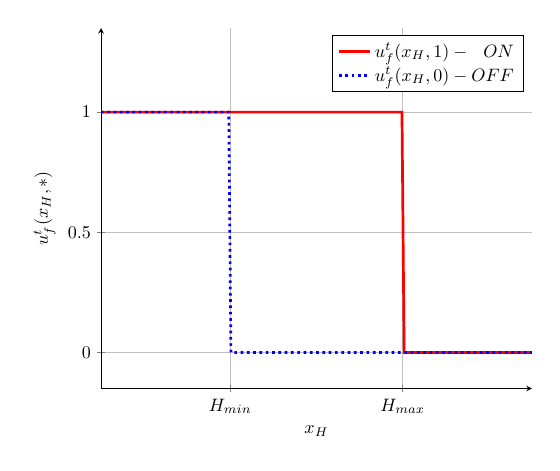
\begin{tikzpicture}[scale=0.65]
        \begin{axis}[
            axis lines = left,
            xlabel = \(x_H\),
            ylabel = {\(u^t_f(x_H,*)\)},
            xmin=-10, xmax=10,
            ymin=-0.15, ymax=1.35,
            grid = major,
            ytick = {0,0.5,1},
            xtick = {-4,4},
            xticklabels = {$H_{min}$,$H_{max}$}
        ]

        %Below the red parabola is defined
        \addplot [
            line width = 1.5pt,
            domain=-10:10, 
            samples=200, 
            color=red,
        ]
        {x< 4};
        \addlegendentry{\(u_f^t(x_H,1) - \ \  ON\)}
        %Here the blue parabola is defined
        \addplot [
            domain=-10:10, 
            samples=200, 
            color=blue,
            line width=1.5pt,
            dotted
            ]
            { x< -4};
            \addlegendentry{\(u_f^t(x_H,0) - OFF\)}
        \end{axis}
        \end{tikzpicture}
        \caption{Fogging Hysteresis}
\end{figure}


Con respecto flujo $u_{f}^{0}$ tomaremos los datos expuestos en la web \cite{WATERMIS30:online}(\emph{Ultra fog preassure water Mist}), este toma el valor de  $w_f \sim  1 \ L/(min\cdot m^2)$ en S.I. $w_f \sim 
(1/60)  \ kg\{H_2O\}/(s\cdot m^2)$. Este es un ficha de espeficicaciones técnicas de un sistema comercial de fogging. 
%
\newline

Teniendo en cuenta que el area del invernadero es $A_f = 50 \ m^2$, obtenemos un flujo de agua hacia la humedad interior de:
%
\begin{gather}
    u_f^0=A_f \cdot w_f = 8.3 \ \times 10^{-1}\ kg\{H_2O\}/s
\end{gather} 

Por otra parte, es necesario pulverizar el vapor en intervalos de $\sim 30s$ ya que de otra manera las gotas de agua en el ambiente no son absorbidos y estos caen al suelo. 
%
De manera que el sistema de nebulización funciona durante $\sim 15s$ y permanece apagado durante otros $\sim 45s$. Dado que el objetivo de la simulación es obtener un perfil anual de funcionamiento y la dinámica del sistema de fogging tiene escala de segundos remplazaremos este funconamiento por su comportamiento medio en un minuto. Entonces en un funcionamiento normal del sistema de fogging el caudal debe ser reducido a un tercio ($15s/45s \to 1/3$) con el objetivo de promediar el tiempo que  apagado y encendido.
\begin{gather}
    u_f^0= \frac{1}{3}A_f \cdot w_f = 2.77 \ \times 10^{-1}\ kg\{H_2O\}/s
\end{gather} 

Con respecto a los limite de funcionamiento de apagado y encendido son tal que la humedad relativa interior no sea inferior de $H_{min}=40\%$ ni superior de $H_{max}=80\%$.
\newline 


En resumen los parámetros de este sistema están recogidos en la Tabla \ref{table:fog_params}.
\newline

\begin{table}[ht!]
    \centering
    \begin{tabular}{|c|c|}
        \hline 
        Parameter & Value \\ \hline \hline
        $\Delta t$ & $1$ minute \\ 
        $u_{f}^{0}$ & $2.77 \times 10^{-1} \ kg\{H_2O\}/s$ \\
        $H_{min}$ & $40\%$ \\
        $H_{max}$ & $60\%$ \\
        \hline 
    \end{tabular}
    \caption{Parámetros de Fogging}\label{table:fog_params}
\end{table}

De manera que podemos ver que en un funcionamiento de $15s+45s=60s$ se descarga una masa de agua de $16 \  kg \{H_2O\}/min$ en una capacidad aproximada de $(40 \sim 90) \ kg \{H_2O\}$ teniendo en cuenta esta capacidad de agua en el aire interior depende de la temperatura en el rango de temperatura $(15 \sim 30)^\circ C$.
\begin{gather}
    (40 \sim 90) \ kg \{H_2O\} \rightleftharpoons (15 \sim 30)^\circ C
\end{gather}



\subsection{Irrigation System }	

El sistema de Irrigación tiene carácter periódico de periodo  un día. Este se activará en intervalos de 5 minutos con paradas de 60 minutos. El tiempo de irrigación dependerá de la radiación acumulada el día anterior. De esta manera, se tiene en cuenta el efecto de la transpiración de las plantas.  
\newline

De manera que definiremos la duracion de irrigación $\Delta t_i$ como:
\begin{gather}
        \Delta t_i = 3 + \lfloor \alpha_{n_i} \cdot x_{AR}\rfloor \hspace{3em} [hours]
\end{gather}
Donde $\lfloor * \rfloor $ es el operador que toma la aproximación entera más cercana por debajo. 
\newline 

Durante el tiempo de funcionamiento $\Delta t_i$ la irrigación esta en funcionamiento durante 5 minutos con un caudal de $i_{flow} = 3L\{H_2O\}/(h\cdot gotero)$, o expresado en S.I. $i_{flow} = 8.33\times 10^{-4} kg\{H_2O\}/(s\cdot gotero)$. 
%
Teniendo en cuenta que un invernadero tiene aproximadamente una densidad de goteros\footnote{Este valor se ha tomado de un invernadero localizado en Meñaka con una superficie de $(80\times40)m^2$ con un total de $1150$ goteros. Podemos estimar que el invernadero de referencia tendrá aproximadamentes $72$ goteros.} de $\rho_g = 1.5 \ goteros/m^2$, y que el area de nuestro invernadero es de $A_f = 50 \ m^2$; podemos obtener el flujo de agua total de todo el invernadero como:
\begin{gather}
    I_{flow}=A_f\cdot\rho_g\cdot i_{flow} = 6.25 \times 10^{-2} kg\{H_2O\}/s
\end{gather} 

La ley de irrigación es una función de la hora del día $h$, y minuto de la hora $m$, además del tiempo adicional de irrigación $\Delta t_i$ y este a su vez  es función de la radiación acumulada $x_{AR}$.
\begin{gather}
    I(\Delta t_i,h,m) = \begin{cases}
            \text{if } (m < m_0) \ \& \ (h \in [9,9+\Delta t_i]) & \Rightarrow I_{flow} \\
            \text{else}  & \Rightarrow 0 
    \end{cases}
\end{gather}

A continuación resumimos los parámetros de funcionamiento en la Tabla \ref{table:irrigation_params}.
\begin{table}[ht!]
    \small
    \centering
    \begin{tabular}{|c|m{5cm}|c|}
        \hline 
        \textbf{Parameter}      & \textbf{Description} & \textbf{Value} \\ \hline \hline
        $\rho_g$       & Densidad de goteros & $1.5 \ goteros/m^2$ \\ \hline
        $A_f$          & Area del invernadero de referencia  & $50 \ m^2$ \\ \hline
        $i_{flow}$     & Flujo de agua por gotero & $8.33 \times 10^{-4}kg\{H_2O\}/(s\cdot goteros)$ \\ \hline 
        $\alpha_{n_i}$ & Coeficiente propocional de horas extra de irrigación por $1MW$& $10^{-6}h/(W/m^2)$   \\ \hline 
        $m_0$          & Minutos de irrigación en una hora & $5 \ mins$ \\ \hline 
        $I_{flow}$     & Flujo total de agua en todo el invernadero & $6.25 \times 10^{-2} kg\{H_2O\}/s$ \\ 
        \hline 
    \end{tabular} 
    \label{table:irrigation_params}
\end{table}

\subsubsection{Cantidades de Referencia}
A grandes rasgos durante un día el número de irrigaciones es de $\sim 5$ veces dando lugar a un consumo diario de agua aproximado (D.W.C) de:
\begin{gather}
    D.W.C \approx 5 \cdot I_{flow}\cdot m_0\cdot\frac{60s}{1min} = 9.3\times 10^{1}  \ kg\{H_2O\}
\end{gather}
 
\subsection{Shading Screens} 

Sistema horario de funcionamiento, por las noches cerrada para aumentar la inercia térmica del invernadero, mientras que por el día solo se abre si el nivel de radiación supera un cierto límite.
\begin{gather}
    u_{scr}^{target}(R_i^{sm}) = \begin{cases}
        0      & \text{if }R_i^{sm} > 50 \ W/m^2 \\
        100   & \text{if }R_i^{sm}  < 50 \ W/m^2 
    \end{cases} 
\end{gather}

Donde es $R_i^{sm}$ de la radiación suavisada de la siguiente manera:
\begin{gather}
    \begin{cases}
        \displaystyle \frac{dR_i^{sm}}{d\tau} & = R_i(\tau) \hspace{1em} \tau \in [0,24]\ hours \\[5pt]
        R_i^{sm}(0)  & = 0
    \end{cases}
\end{gather}

Por otra parte, con el fin de que la velocidad de las pantallas de sombreo sea limitada a $v_{src}=100\%/0.5h$ (el sistema tardara media hora en cerrar o abrir completamente desde el estado opuesto).
\begin{gather}
    \begin{cases}
        \displaystyle \frac{du_{scr}}{d\tau} & =  v_{src}\tanh(u_{scr}^{target}(R_i)-u_{scr}) \\
        du_{scr}(0) & =  0
    \end{cases}
\end{gather}
\subsection{Heating System}

El sistema de calefacción actua de la misma manera que el fogging pero teniendo en cuenta el valor de la temperatura. Este es un controlador para el el limite inferior de tempeartura como extremo inferior. Matemáticamente se puede expresar como: 
\begin{gather}\label{eq:HeatLaw}
    u^{t}_{heat}(x_H,u^{t-\Delta t}_{heat}) = \begin{cases}
        0 & \text{if } T_i > T_{max} \\
        u^0_{heat} & \text{if } T_i < T_{min} \\
        u^{t-\Delta t}_{heat} & \text{if } x_T \in [T_{min},T_{max}]
    \end{cases} 
\end{gather}

\begin{table}[ht!]
    \centering
    \begin{tabular}{|c|c|}
        \hline 
        Parameter & Value \\ \hline \hline
        $\Delta t$ & $5 \ mins$ \\
        $u^0_{heat}$ & $10^{7} \ W$ \\
        $T_{min}$ & $12 ^\circ C$\\
        $T_{max}$ & $20 ^\circ C$ \\
        \hline 
    \end{tabular} 
\end{table}

A contiuación presentamos una representación gráfica de la ecuación \eqref{eq:HeatLaw} en la Figura \ref{figure:HeatLaw}.

\begin{figure}[ht!]
    \centering
    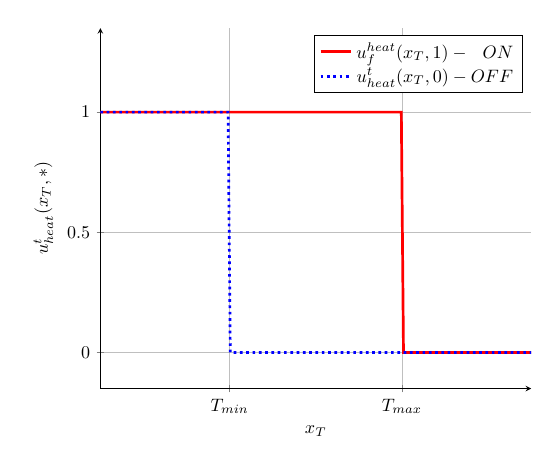
\begin{tikzpicture}[scale=0.65]
        \begin{axis}[
            axis lines = left,
            xlabel = \(x_T\),
            ylabel = {\(u^t_{heat_{}}(x_T,*)\)},
            xmin=-10, xmax=10,
            ymin=-0.15, ymax=1.35,
            grid = major,
            ytick = {0,0.5,1},
            xtick = {-4,4},
            xticklabels = {$T_{min}$,$T_{max}$}
        ]

        %Below the red parabola is defined
        \addplot [
            line width = 1.5pt,
            domain=-10:10, 
            samples=200, 
            color=red,
        ]
        {x< 4};
        \addlegendentry{\(u_f^{heat}(x_T,1) - \ \  ON\)}
        %Here the blue parabola is defined
        \addplot [
            domain=-10:10, 
            samples=200, 
            color=blue,
            line width=1.5pt,
            dotted
            ]
            { x< -4};
            \addlegendentry{\(u_{heat}^t(x_T,0) - OFF\)}
        \end{axis}
        \end{tikzpicture}
        \caption{Fogging Hysteresis}
        \label{figure:HeatLaw}
\end{figure}

\subsection{Sistema de Ventilación}

El sistema de ventilación tiene dos modos de funcionamiento dependiendo si estamos de día o de noche. De día el sistema de ventilación tiene como objetivo el mantener la temperatura en ele interior por debajo del la “Temperatura de Calefacción”, usualmente con un valor de 18ºC. Este actúa de manera proporcional empezando desde la temperatura de calefacción y terminando con la apertura máxima de la ventana. 
%
\begin{gather}
    u_{win}^{day}(T_i) = \begin{cases}
        0  & \text{if } T_i < T_{ven} \\ 
        100 \cdot (T_i - T_{ven}^{min})/(T_{ven}^{max} - T_{ven}^{max}) & \text{if } T_i \in  T_{ven}^{min} \\
    \end{cases}
\end{gather} 

Con el fin de evitar ruido en el funcionamiento de las ventanas no se utiliza la señal de la temperatura interior directamente sino una media móvil. 
\newline

Por la noche el sistema de ventilación entiende que el set-point superior de $18^\circ C$ esta controlado ya que la temperatura exterior esta muy lejos de este valor. Es por ello que el sistema de ventilación no actua para controlar la temperatuara, sino para control los niveles de humedad. Cuando la temperatura baja, la concentración de vapor de agua en el aire también disminuye. Esto hace que sea más fácil alcanzar niveles de humedad relativa alto, es por ello que para evitar la condensación en las paredes del invernadero se utiliza la ventilación para que la humedad interior y exterior se homogenizen.
\newline

De noche la ley de control se puede escribir como:
\begin{gather}
    u_{win}^{night}(H_i) = \begin{cases}
        0  & \text{if } H_i < H_{ven} \\ 
        10 \cdot (H_i - H_{ven}^{min})/(H_{ven}^{max} - H_{ven}^{max}) & \text{if } H_i \in  H_{ven}^{min} \\
        \end{cases}
\end{gather}

Con el fin de tener en cuenta el cambio de la salida y puesta de sol provocado por los cambios de estaciones, utilizaremos la radiación como método de cambio de control. De manera que: 
\begin{gather}
    u_{win}(R_i,T_i,H_i) = 
    \begin{cases}
        u_{win}^{night}(H_i) & R_i \leq 50 W/m^2 \\[5pt]
        u_{win}^{day}(T_i)   & R_i > 50 W/m^2
    \end{cases}
\end{gather}

\subsection{Sistema de Radiación Artificial}

El sistema de radiación artificial se activa si la radiación acumulada interior $AR_i$ es inferior a un threshold $AR_i^{min}$. Este se activa a partir de las $22:00$ horas y además la duración de funcionamiento es proprocional al gap de radiación acumulada. Esta ley se cumple hasta un máximo de duración de $d_{max}=4$ horas.

De esta manera si llamamos $\R$ a la radiación acumulada hasta las $22:00$
\begin{gather}
    \R = \frac{1}{(3600*24) s}\int_{t}^{t-3600} R_i(\tau)d\tau
\end{gather}
Entonces la duración se puede calcular como:
\begin{gather}
    \Delta t_r(\R) =        
    \begin{cases}
        0 & \R > \R^{min} \\
        \beta(\R-\R^{min}) & \R \in [\R^{min},\R^{max}] \\
        d_{max} \\
    \end{cases}
\end{gather}
Este valor se calcula cada día a las $22:00$.

\begin{figure}[ht!]
    \centering
    \begin{tikzpicture}[scale=0.65]
        \begin{axis}[
            axis lines = left,
            xlabel = \(\R\),
            ylabel = {\(\Delta t_r (\R) \)},
            xmin=-10, xmax=10,
            ymin=-1, ymax=10,
            grid = major,
            ytick = {0,8},
            xtick = {-4,4},
            xticklabels = {$\R_{min}$,$\R_{max}$},
            yticklabels = {$0$,$d_{max}$}
        ]

        %Here the blue parabola is defined
        \addplot [
            domain=-10:10, 
            samples=200, 
            color=blue,
            line width=1.5pt,
            dotted
            ]
            { (x>-4)*(x< 4)*(x+4) + (x>=4)*8};
        \end{axis}
        \end{tikzpicture}
        \caption{Duration of Lighting System}
        \label{figure:HeatLaw}
\end{figure}

Donde la radiación acumulada máxima  $\R^{max}$ donde el valor de la duración se satura es $\R= d_{max}/\beta + \R^{min}$.
\begin{gather}
    u_{ar}(\Delta t_r,h,m) = \begin{cases}
            \text{if } (m < m_0) \ \& \ (h \in [22,22+\Delta t_r]) & \Rightarrow u_{ar}^0 \\
            \text{else}  & \Rightarrow 0 
    \end{cases}
\end{gather}



\section{Datos de Entrada}

Esta simulación se a realizado con mezcla de datos climáticos tomados de la estación meteorológica (Radiación, Temperatura y Velocidad del viento) y una señal de humedad relativa de la estación meteorológica cercana. Estos datos tienen un tiempo de muestro de diez minutos empezando el 01/01/2019 00:00:00 y terminando en 31/12/2019 00:00:00



\bibliographystyle{apalike}
\bibliography{bib}
\end{document}